\begin{figure}
  \setlength{\unitlength}{\textwidth}
  \begin{picture}(1,0.3)(0,0.8)
    % % %90
    \put(0.025,0.83){\includegraphics[width=0.5\unitlength]{../FnP/gnuplot/vel_time_history_60_0.075.eps}}
    \put(0.495,0.83){\includegraphics[width=0.5\unitlength]{../FnP/gnuplot/vel_time_history_165_0.175.eps}}
    
    \put(0.03,0.95){ $\frac{V}{D}$} 	
    % \put(0.56,1.02){ $\frac{V}{D}$}
 	
    \put(0.25,0.805){ $\frac{tU}{D}$} 	
    \put(0.73,0.805){ $\frac{tU}{D}$}

    \put(0.095,1.03){(a)}
    \put(0.565,1.03){(b)}

  \end{picture}

  \caption{Time histories of velocity at two different $\zeta$ and $U^*$ which produce the same mean power ($1.2\times10^{-3}$). Data presented using QSS assumption, (a) at $\ustar=60$ and $\zeta=0.075$, (b) at $\ustar=165$ and $\zeta=0.175$ at Re=165. Shedding is evident in both signals as a high frequency fluctuation but the amplitude of the slower fluctuations remains constant in both cases.}
    \label{fig:time_hostory_velocity_same_power}
\end{figure}